\documentclass[10pt,a4paper]{article}
\usepackage[bindingoffset=0.2in,%
            left=2.5cm,right=2cm,top=2.7cm,bottom=1in,%
            footskip=.25in]{geometry}
\usepackage[utf8]{inputenc}
\usepackage[ngerman]{babel}
\usepackage{amsmath, amsfonts, amssymb}
\usepackage{scrpage2}
\usepackage{color}
\usepackage{titlesec}
\pagestyle{scrheadings}
\usepackage{ulem, contour}
\usepackage{multicol}
\usepackage{hyperref}
\usepackage{listings}
\usepackage{pdfpages}
\usepackage{tabularx}
\usepackage{subcaption}
\usepackage{float}
\usepackage{scrextend}
\usepackage{enumerate}
\usepackage[bottom, splitrule]{footmisc}
\usepackage{multirow}
\usepackage{csquotes}

\usepackage[style=authoryear, backend=biber]{biblatex}
\addbibresource{bibliography.bib}

\DeclareFixedFont{\ttb}{T1}{txtt}{bx}{n}{12} % for bold
\DeclareFixedFont{\ttm}{T1}{txtt}{m}{n}{12}  % for normal

\renewcommand{\ULdepth}{1.8pt}
\contourlength{0.8pt}

\newcommand{\cul}[1]{%
  \uline{\phantom{#1}}%
  \llap{\contour{white}{#1}}%
}

\graphicspath{
    {Images/}
}

\newrobustcmd*{\parentexttrack}[1]{%
  \begingroup
  \blx@blxinit
  \blx@setsfcodes
  \blx@bibopenparen#1\blx@bibcloseparen
  \endgroup}

\AtEveryCite{%
  \let\parentext=\parentexttrack%
  \let\bibopenparen=\bibopenbracket%
  \let\bibcloseparen=\bibclosebracket}

\definecolor{gray}{rgb}{0.33, 0.33, 0.33}
\definecolor{greengreen}{rgb}{0.0, 0.56, 0.0}
\definecolor{fgreen}{rgb}{0.13, 0.55, 0.13}
\definecolor{grellow}{rgb}{0.68, 1.0, 0.18}
\definecolor{orange}{rgb}{1.0, 0.49, 0.0}
\definecolor{deepblue}{rgb}{0,0,0.5}
\definecolor{deepred}{rgb}{0.6,0,0}
\definecolor{deepgreen}{rgb}{0,0.5,0}

\usepackage{pifont}

\newcommand{\cmark}{\ding{51}}%
\newcommand{\xmark}{\ding{55}}%
\newcommand{\wontfix}{\rlap{$\square$}{\large\hspace{1pt}\xmark}}


\newcommand{\vnr}{1}
\newcommand{\anr}{1}

\ihead{}
\ohead{Anfängerpraktikum 2}
\chead{Versuch \vnr, Abgabe \anr : Strom- \& Spannungsmessung}
\cfoot{\pagemark}
\setheadsepline{.5pt}
\setlength\parindent{0pt}

\begin{document}

\begin{multicols}{2}
\begin{labeling}{Versuch-Nr.:}
\item[\textcolor{white}{x}Protokollant:\hspace{38pt}] \cul{Name} \wontfix
\item[\textcolor{white}{x}Zusammenarbeit\footnotemark mit:] \cul{Name} $\square$
\item[\textcolor{white}{x}Datum:\hspace{62pt}] \cul{\today}

\columnbreak

\item[Kurs: \hspace{27pt}] \cul{Anfängerpraktikum 2}
\item[Assistent: \hspace{8.7pt}] \cul{Name}
\item[Versuch-Nr.:] \underline{\vnr}
\end{labeling}
\end{multicols}

\footnotetext{Zusammenarbeit meint Unterhalten über die Messergebnisse und Ideenaustausch. Unsere Protokolle sind jeweils eigene Werke.}

\begin{figure}[h]
\hspace{-0.5cm}\centerline{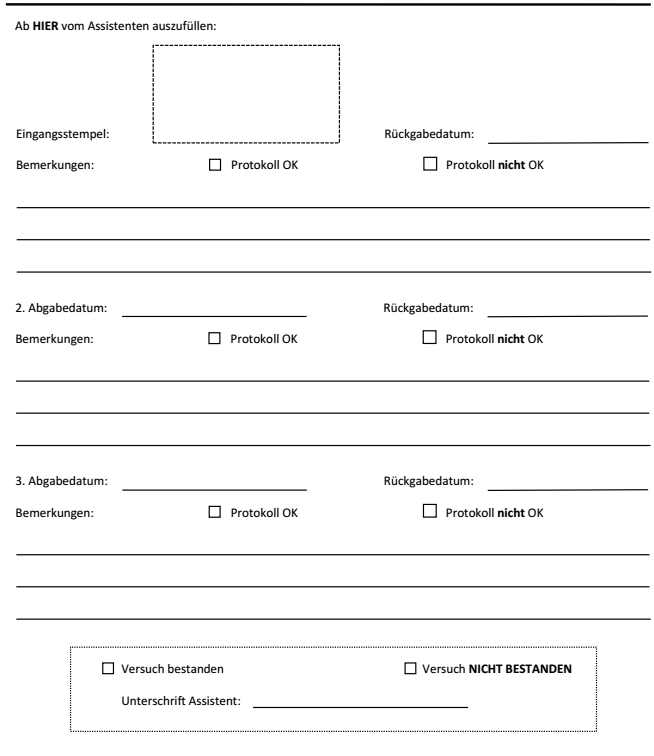
\includegraphics[width=1.1\linewidth , height=19cm]{Deckblatt_rest}}
\end{figure}

\newpage

\tableofcontents

\vspace{10pt}

\section{Aufgabenstellung}
\begin{flushleft}
Der Versuch Nr. \vnr \hspace{1pt} \glqq Strom- und Spannungsmessung\grqq\hspace{1pt} behandelt das Messen bestimmter Größen und Ermitteln einer weiteren Größe auf Basis dieser. Konkret werden in diesem Versuch die Spannung \textit{U} und Stromstärke \textit{I} gemessen, um dadurch die Größe eines unbekannten Widerstandes zu ermitteln.

Dabei ist wie folgt vorzugehen:
\begin{enumerate}[I]
\item Messen von Spannung und Stromstärke, die Tabelle~\ref{tab:messerg} ausfüllen.

\item Die Messergebnisse (u.a. graphisch) auswerten.

\item Diskussion der Ergebnisse. Dazu insbesondere auf Messung zehn und elf eingehen.
\end{enumerate}
\end{flushleft}

\subsection{Physikalischer Hintergrund}
\begin{flushleft}
In diesem Versuch wird der Zusammenhang zwischen verschieden physikalischen Größen thematisiert. Konkret werden dabei die Größen Spannung, Stromstärke, Widerstand und Leistung betrachtet.

Hierbei hängen diese Größen im Stromkreislauf insofern zusammen, dass der Wert des Produkt aus Spannung und Stromstärke der Leistung entspricht ($P = U \cdot I$) und der Quotient beschreibt den Wert des Widerstandes ($R = \frac{U}{I}$).
\end{flushleft}

\section{Messmethoden}
\begin{flushleft}
Im Folgenden ist der Versuchsaufbau, sowie der Schaltplan für den Versuch beschrieben. Hierbei wurde der Schaltplan in zwei Pläne \textit{A} und \textit{B} getrennt, um eine besssere Übersicht zu gewährleisten. Im weiteren Verlauf des Protokolls werden die Schaltpläne mit \textit{Schaltung A} und \textit{Schaltung B} bezeichnet.
\end{flushleft}

\subsection{Versuchsaufbau}
\begin{flushleft}
Für unser Experiment benötigen wir folgende Materialen:

\begin{itemize}
\item Einen Widerstand (unbekannter Größe)
\item Eine Spannungsquelle
\item Ein Amperemeter
\item Ein Voltmeter
\item (mehrere) Kabel
\end{itemize}

Hierbei verwenden wir jeweils ein Multimeter für Amperemeter und Voltmeter. Zusätzlich haben wir ein Schiebepotentiometer eingebaut, um die Spannung während des Versuches zu ändern.
\end{flushleft}

\subsection{Schaltpläne}
\begin{figure}[H]
\centering
\begin{subfigure}[c]{0.5\textwidth}
\vspace{10pt}
\centering
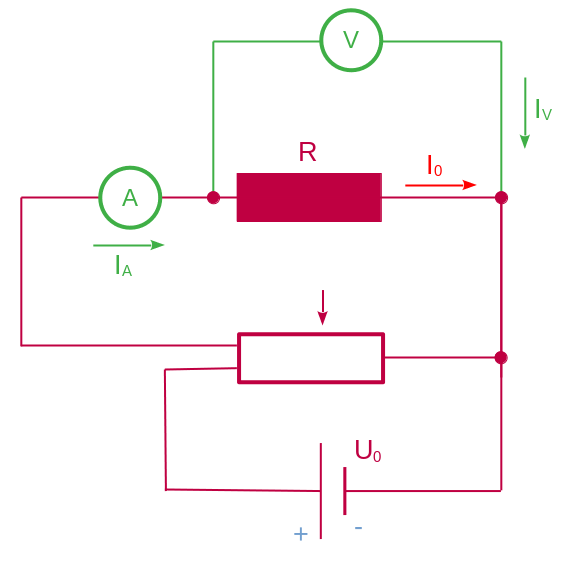
\includegraphics[scale=0.35]{Schaltung_A}
\subcaption{Schaltung A}
\end{subfigure}%
\begin{subfigure}[c]{0.5\textwidth}
\centering
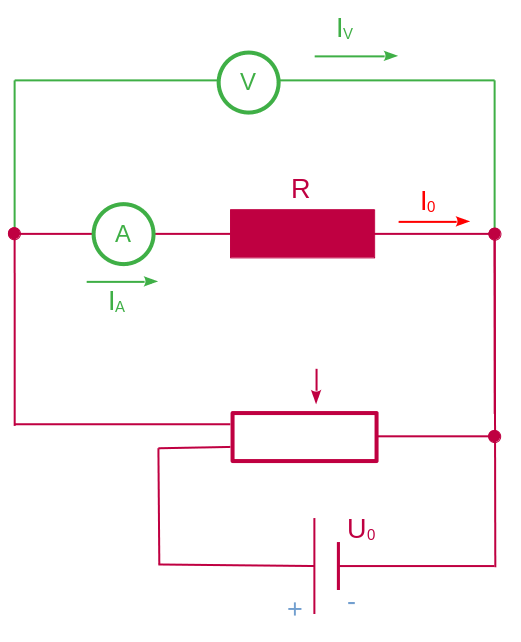
\includegraphics[scale=0.35]{Schaltung_B}
\subcaption{Schaltung B}
\end{subfigure}%
\caption[Schaltpläne]{Schaltpläne}
\label{fig:schaltungen}
\end{figure}

\begin{flushleft}
\textbf{Erklärung der Größen:}

\begin{itemize}
\item[$I_A$:] Der Strom, der am Amperemeter abfällt.
\item[$I_V$:] Der strom, der am Voltmeter abfällt.
\item[$I_0$:] Der Strom, der am Widerstand abfällt.
\item[$U_0$:] Spannugn, die and der Stromquelle angelegt ist.
\end{itemize}
Auf Grund der Parallelschaltung des Widerstandes und des Voltmeters fällt am Widerstand nicht der gesamte Strom am Widerstand ab. Es gilt $I_{ges} = I_0 + I_V$ für die parallelschaltung von Widerständen (Reihenschaltung: $I = konst$).
\end{flushleft}

\section{Versuchsdurchführung}
\begin{flushleft}
Wir beginnen mit der Durchführung, indem wir die \textbf{Schaltung A} aufbauen. Wir messen zehn mal, wobei wir nach jeder Messung die Spannung mit dem Schiebepotentiometer erhöhen. Anschließend bauen wir den Aufbau zu \textbf{Schaltung B} um. Bei diesem Aufbau messen wir ein mal mit der letzten Einstellung des Schiebepotentiometer bei Schaltung A. Die Messwerte werden in die Tabelle~\ref{tab:messerg} eingetragen.
\end{flushleft}

\section{Versuchsergebnisse}
\hspace{-4pt}
\begin{table}[H]
\centering
\caption[Messergebnisse]{Messergebnisse\footnotemark}
\label{tab:messerg}
\scriptsize
% \begin{tabularx}{\textwidth}{|R|R|R|R|R|R|R|R|R|R|R|R|R|R|}
\centerline{
\begin{tabular}{|c|c|c|c|c|c|c|c|c|c|c|c|c|c|}
\hline
$U (V)$ & $U_{max} (V)$ & $\Delta U (V)$ & $\Delta U / U$ & $I (A)$ & $I_{max} (A)$ & $\Delta I (A)$ & $\Delta I / I$ & $R (\Omega)$ & $\Delta R (\Omega)$ & $\Delta R / R$ & $P (W)$ & $\Delta P (W)$ & $\Delta P / P$ \\
\hline
0.61 & 1 & 0.01 & 0.017 & 0.027 & 0.03 & $3\cdot 10^{-4}$ & 0.012 & 22.593 & 0.622 & 0.028 & 0.017 & $4.53\cdot 10^{-4}$ & 0.02 \\ 
\hline
0.76 & 1 & 0.01 & 0.014 & 0.034 & 0.1 & 0.001 & 0.03 & 22.353 & 0.952 & 0.043 & 0.026 & 0.002 & 0.04 \\ 
\hline
1 & 1 & 0.01 & 0.01 & 0.044 & 0.1 & 0.001 & 0.023 & 22.728 & 0.744 & 0.033 & 0.044 & 0.002 & 0.03 \\ 
\hline
1.2 & 3 & 0.03 & 0.025 & 0.052 & 0.1 & 0.001 & 0.02 & 23.077 & 1.021 & 0.045 & 0.063 & 0.003 & 0.04 \\ 
\hline
1.5 & 3 & 0.03 & 0.02 & 0.066 & 0.1 & 0.001 & 0.016 & 22.728 & 0.799 & 0.036 & 0.099 & 0.004 & 0.03 \\ 
\hline
2.05 & 3 & 0.03 & 0.015 & 0.09 & 0.1 & 0.001 & 0.012 & 22.778 & 0.587 & 0.026 & 0.185 & 0.005 & 0.02 \\ 
\hline
2.35 & 3 & 0.03 & 0.013 & 0.105 & 0.3 & 0.003 & 0.029 & 22.381 & 0.926 & 0.042 & 0.247 & 0.011 & 0.04 \\ 
\hline
2.8 & 3 & 0.03 & 0.011 & 0.125 & 0.3 & 0.003 & 0.024 & 22.4 & 0.778 & 0.035 & 0.35 & 0.013 & 0.03 \\ 
\hline
3.2 & 10 & 0.1 & 0.032 & 0.14 & 0.3 & 0.003 & 0.022 & 22.858 & 1.205 & 0.053 & 0.448 & 0.024 & 0.05 \\ 
\hline
4.5 & 10 & 0.1 & 0.023 & 0.2 & 0.3 & 0.003 & 0.015 & 22.5 & 0.838 & 0.038 & 0.9 & 0.034 & 0.03 \\ 
\hline
4.7 & 10 & 0.1 & 0.022 & 0.2 & 0.3 & 0.003 & 0.015 & 23.5 & 0.853 & 0.037 & 0.94 & 0.035 & 0.03 \\ 
\hline
\end{tabular}
}
\end{table}

\footnotetext{Die Messergebnisse wurden auf die 3. Nachkommastelle gerunded.}

\begin{flushleft}
Die Tabelle \ref{tab:messerg} zeigt die Messergebnisse, sowie die berechneten Werte für Widerstand (\textit{R}, in Ohm) und Leistung (\textit{P}, in Watt). Zudem sind jeweils der absolute und relative Fehler der Messung eingetragen. Die verwendeten Multimeter haben dabei nach Angabe des Gerätes eine Genauigkeit von $\pm1\%$.

Auf Grund des Zusammenhangs des Widerstands mit $R = \frac{U}{I}$ besteht eine systematische Fehlerfortpflanzung, die mit der Größtfehlermethode berechnet wird. Der relative Fehler wird im Allgemeinen berechnet mit:
\begin{equation*}
\Delta y = \frac{\delta y}{\delta x_1} \Delta x_1 + \frac{\delta y}{\delta x_2} \Delta x_2 + ...
\end{equation*}

Für den Widerstand und die Leistung berechnen wir den absoluten Fehler dann konkret durch:
\begin{align*}
\Delta R &= \vert\frac{1}{I}\vert \cdot \Delta U + \vert\frac{U}{I^2}\vert \cdot \Delta I \\
\Delta P &= I \cdot \Delta U + U \cdot \Delta I \\
\end{align*}
\end{flushleft}

\begin{figure}[H]
\centering
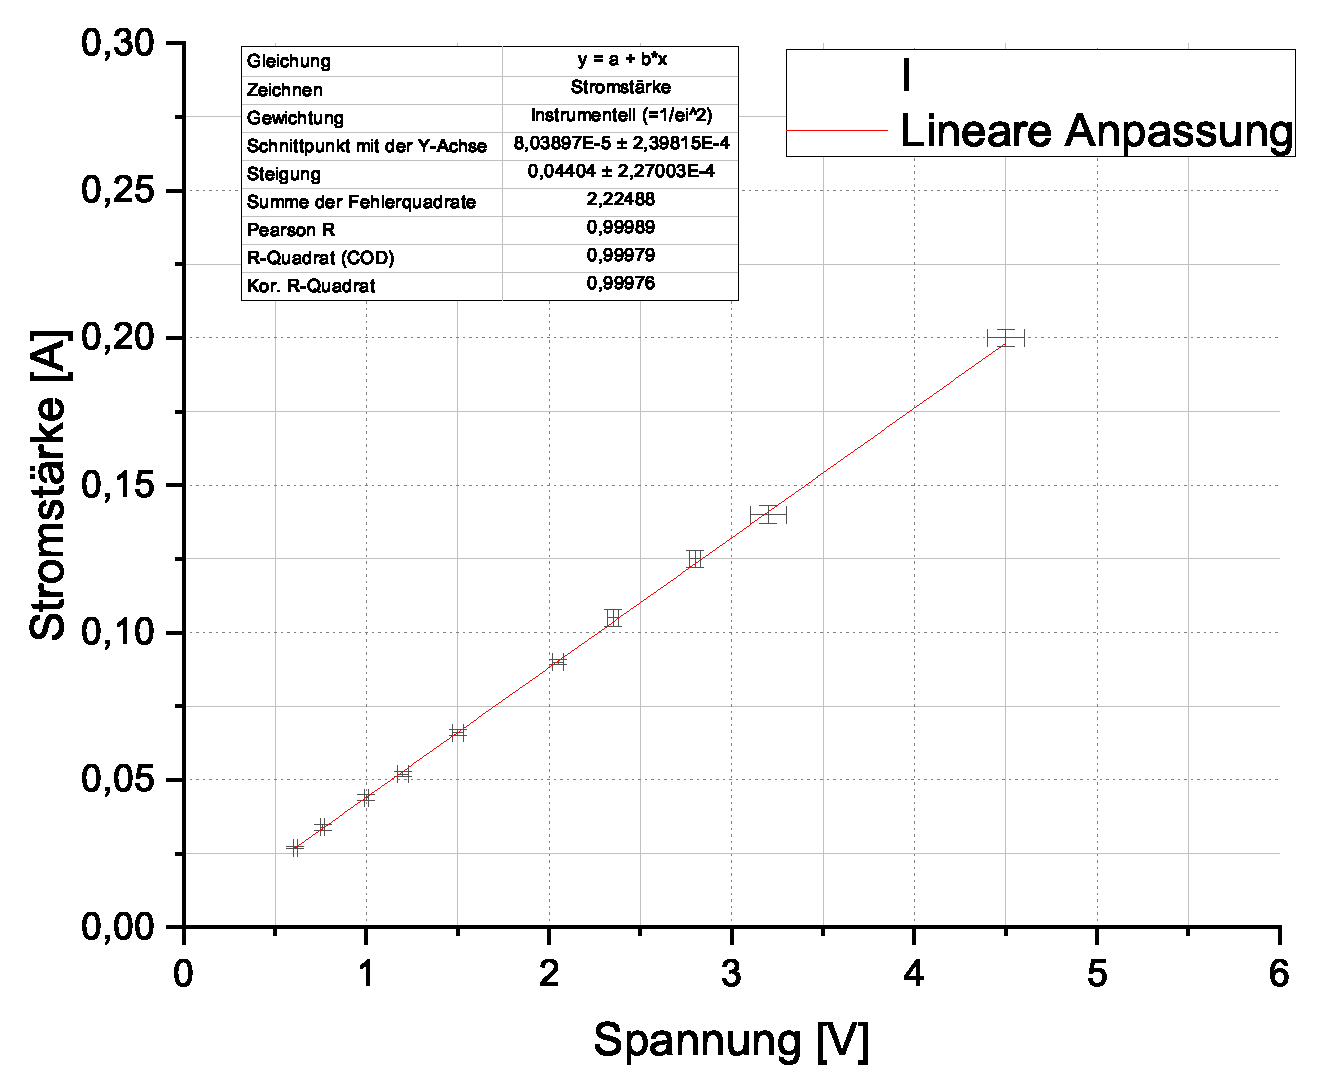
\includegraphics[scale=0.5]{Graph1}
\caption[Graph: Spannung \& Strom]{Graphische Darstellung der Messdaten zu Spannung und Stromstärke}
\label{fig:SpannStrom}
\end{figure}

\begin{figure}[H]
\centering
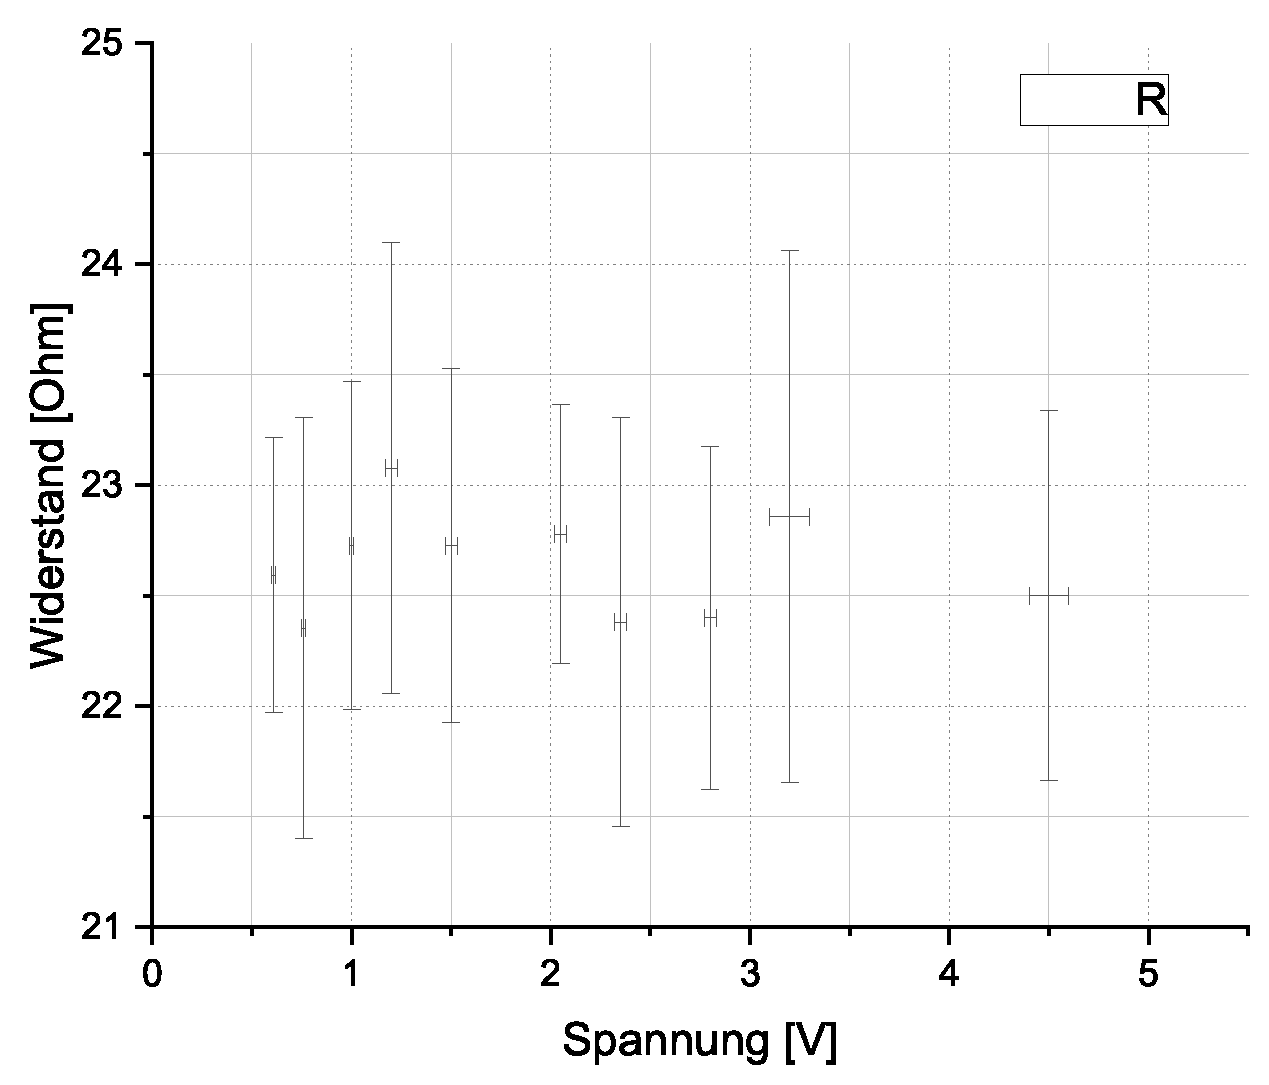
\includegraphics[scale=0.5]{Graph2}
\caption[Graph: Spannung \& Strom]{Graphische Darstellung der Messdaten zu Spannung und Widerstand}
\label{fig:SpannWid}
\end{figure}

\begin{figure}[H]
\centering
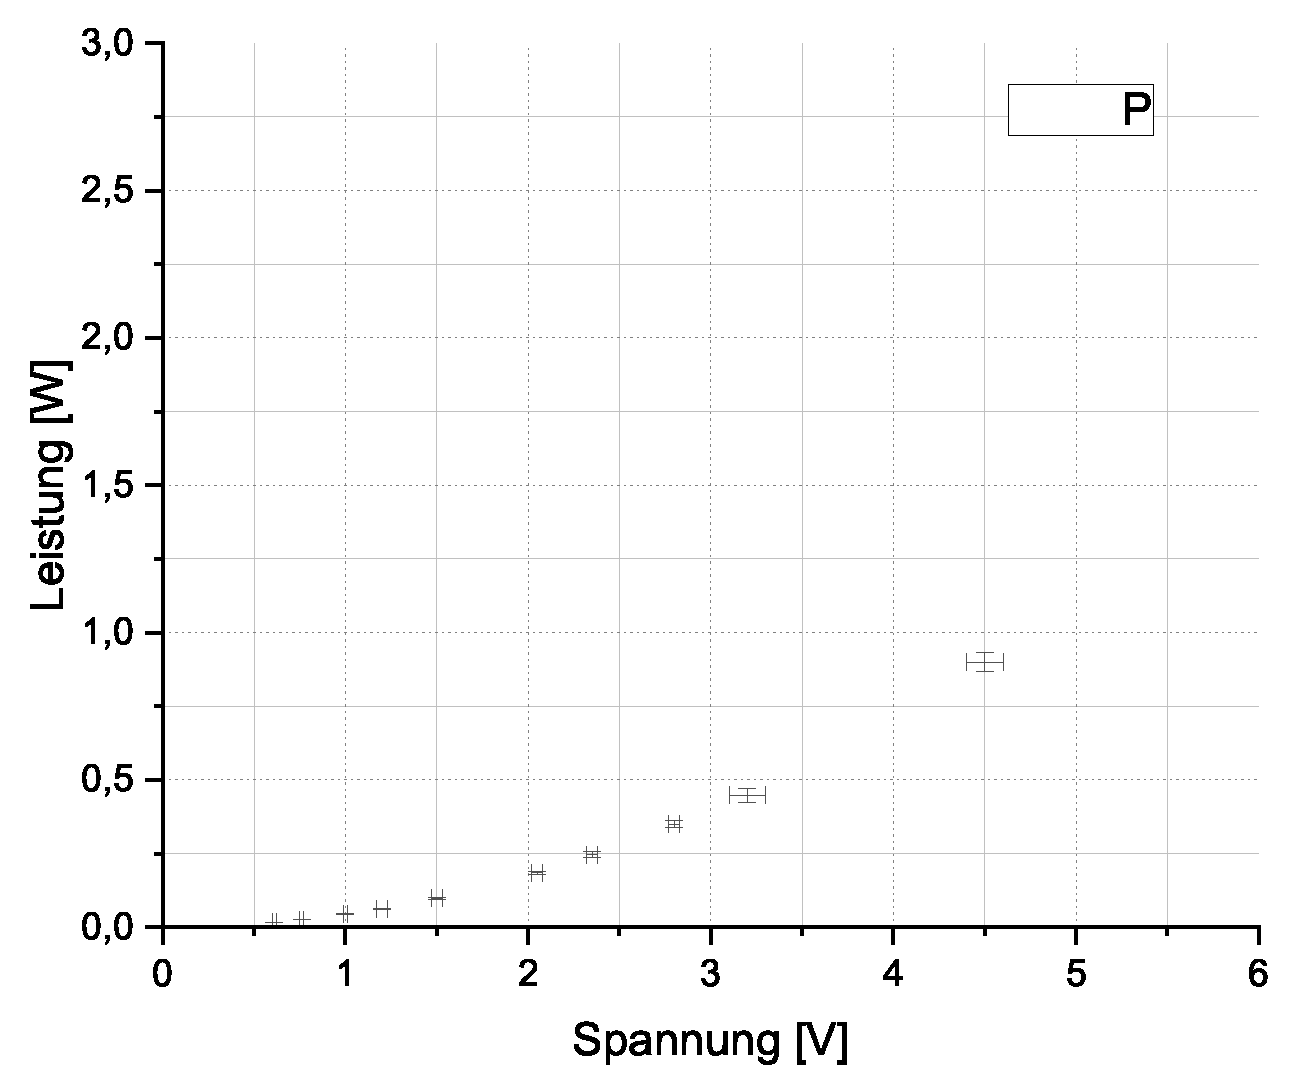
\includegraphics[scale=0.5]{Graph3}
\caption[Graph: Spannung \& Strom]{Graphische Darstellung der Messdaten zu Spannung und Leistung}
\label{fig:SpannPow}
\end{figure}

\begin{flushleft}
Für die graphische Darstellung der Messwerte wurden nur die ersten zehn Messungen herangezogen. Die elfte Messung wurde mit \textbf{Schaltung B} (Siehe Abbildung \ref{fig:schaltungen}) und nicht wie die ersten zehn mit \textbf{Schaltung A} gemessen und kann somit hier nicht in diesem Umfang mit diesen verglichen werden!
\end{flushleft}

\subsection{Diskussion der Messergebnisse}
\begin{flushleft}
Die Messergebnisse zeigen, dass die Spannung \textit{U} und Stromstärke \textit{I} linear zusammenhängen (Graph Abbildung \ref{fig:SpannStrom}). Im Gegenensatz dazu stehen Spannung \textit{U} und Leistung \textit{P} quadratisch zusammen (Graph Abbildung \ref{fig:SpannPow}), was durch $P = U \cdot I = R \cdot I^2$ auch erkenntlich ist.

Aus unseren Messergbnissen können wir weiterhin den Mittelwert der Widerstandswerte der Messungen bilden. Diesen erhalten wir, indem wir die Summe der Widerstandswerte durch die Anzahl der Messungen teilen. Hierbei berücksichtigen wir wieder nur die ersten zehn Messungen, die mit \textbf{Schaltung A} gemessen wurden.
\end{flushleft}

\begin{figure}[h]
\centering
\begin{subfigure}[c]{0.5\textwidth}
\subcaption{Berechnung des Mittelwertes}
\begin{align*}
\varnothing R &= \frac{\sum R_i}{n} \\
&\approx \frac{226.396 \Omega}{10} \\
&\approx 22.64 \Omega \\
\end{align*}
\end{subfigure}%
\begin{subfigure}[c]{0.5\textwidth}
\subcaption{Berechnung des Standardfehlers\footnotemark}
\begin{align*}
\sigma_{\bar{x}} &= \frac{\sigma}{\sqrt{n}} = \sqrt{\frac{\sum(R_i - \varnothing R)^2}{n-1}} \cdot \frac{1}{\sqrt{n}} \\
&= \frac{0.23615 \Omega}{\sqrt{10}} \\
&\approx 0.075 \Omega
\end{align*}
\end{subfigure}%
\end{figure}

\footnotetext{Die Berechnung des Standardfehler erfolgt auf Basis der Formeln aus \href{https://de.wikipedia.org/wiki/Standardfehler}{Wikipedia}, einem \href{https://www.easycalculation.com/de/statistics/standard-deviation.php}{Standardabweichungsrechner}, sowie einer \href{https://www.scribbr.de/statistik/standardfehler/}{Anleitung} zur Berechnung.}

\begin{flushleft}
Dabei beträgt der Mittelwert der berechneten Widerstandswerte $\approx (22.64 \pm 0.075) \Omega$ (Abbildung \ref{fig:SpannWid} zeigt die berechneten Werte des Widerstandes je Messung). Im Vergleich dazu beträgt der Wert des Widerstandes nach der linearen Regression $R \approx (22.707 \pm 0.117)\Omega$\footnote{$\Delta R_{Regression} = \pm \frac{\Delta b}{|b^2|}$, mit Steigung b der Regression.}. Diese Werte sind sich recht nahe und es ist davon auszugehen, dass die tatsächliche Größe des Widerstandes bei $\approx 22.7 \Omega$ liegt.

Die Messergebnisse zu Spannung und Stromstärke (Siehe auch Tabelle \ref{tab:messerg}) zeigen zudem, dass die verschiedenen Schaltungen \textbf{Schaltung A} und \textbf{Schaltung B} (Siehe Tabelle \ref{fig:schaltungen}) einen Einfluss auf die Werte haben. Dies ist anhand Messung zehn und Messung elf zu erkennen. Bei Messung zehn wurde dabei nach \textbf{Schaltung A} gemessen, bei Schaltung elf nach \textbf{Schaltung B}. Die Messung zeigt, dass der Wert der Spannung um $0.2V$ abweicht. Dies ist dadurch zu erklären, dass die Messgeräte selbst einen Widerstand eingebaut haben, um überhaupt Stromstärke und Spannung messen zu können.
\end{flushleft}

\begin{table}[h]
\centering
\caption[Fallunterscheidung]{Fallunterscheidung der Schaltungen und unbekannten Widerstände\footnotemark}
\label{tab:Fallunterscheidung}
\begin{tabular}{|c|c|c|c|}
\hline
& & Strom & Spannung \\
\hline
\multirow{2}{*}{Messung A} & $R_X \to R_A$ & \cmark & \cmark  \\
\cline{2-4}
& $R_X \to R_V$ & \xmark & \cmark \\
\hline
\multirow{2}{*}{Messung B} & $R_X \to R_A$ & \cmark & \xmark \\
\cline{2-4}
& $R_X \to R_V$ & \cmark & \cmark \\
\hline
\end{tabular}
\end{table}

\footnotetext{Es bezeichnet $R_x$ den unbekannten Widerstand, $R_A$ den Widerstand am Amperemeter und $R_V$ den Widerstand am Voltmeter.}

\begin{flushleft}
Eine Messung mit \textbf{Schaltung A} ermöglicht eine \textbf{korrekte Spannungsmessung}. Im Gegensatz dazu ermöglich \textbf{Schaltung B} eine \textbf{korrekte Strommessung}.

Generell gelten die Gesetze der \textit{Reihen- und Parallelschaltung von Widerständen} auch bei der Messung von Stromstärke und Spannugn am Widerstand. Dadurch werden u.U. Fehler begünstigt. Die Tabelle \ref{tab:Fallunterscheidung} zeigt, wie sich das Größenverhältnis des unbekannten Widerstandes zu den eingebauten Widerständen der Messinstrumente auf die Messgenauigkeit auswirkt. Ein Haken (\cmark) bedeutet, dass sich die Fehler der Messung in den angegebenen Grenzen hält, ein Kreuz (\xmark) bedeutet, dass die Fehler die Fehlergrenzen überschreiten können.

\textbf{Schaltung A} ist eine korrekte Spannungsmessung, weshalb die gemessene  Fehlerspannung in den Fehlergrenzen bleibt. Analog gilt dies für \textbf{Schaltung B} als korrekte Strommessung. Bei beiden Schaltungen hängt jedoch von dem Größenverhältnis des unbekannten Widerstandes zum Widerstandes des Messgerätes ab, ob die jeweils andere Größe im Fehlerrahmen gemessen werden kann.

Im Fall, dass der unbekannte Widerstand $R_X$ gegen den Widerstand des Amperemeters $R_A$ läuft, also eher klein(er) ist, ist auch eine korrekte Strommessung in \textbf{Schaltung A} möglich. Dies ist dadurch zu erklären, dass bei kleinem unbekannten Widerstand ein großer Strom fließt und somit nur ein relativ kleiner Teil dessen vom Voltmeter benötigt wird, um die Spannung anzuzeigen. Bei großem unbekannten Widerstand ($R_X \to R_V$) fließt wiederum ein kleiner Strom, wodurch der verursachte Stromfehler des Spannungsmessgerätes größer wird. Bei \textbf{Schaltung B} verhält sich die Messgenauigkeit für die Spannung genau umgedreht. Hier kann bei großem unbekannten Widerstand $R_X \to R_V$ auch die Spannung im Fehlerbereich gemessen werden, da bei großem Widerstand ein kleiner(er) Strom fließt und somit nur ein kleiner(er) Spannungsfehler entsteht. Dieser Spannungsfehler erhöht sich, je mehr sich der unbekannte Widerstand dem Wert des Widerstandes am Amperemeter nähert und verursacht dadurch eine ungenauere Messung der Spannung am Voltmeter \parencite[vgl.][]{SpannStrom}.

Bei diesem Versuch haben wir ermittelt, dass der Widerstand eine Größe von rund $22.7 \Omega$ besitzt. Der Innenwiderstand des Multimeters als Voltmeters beträgt in den von uns verwendeten Wertebereichen $5k\Omega$, weshalb eine Messung mit \textbf{Schaltung A} eher geeignet ist.
\end{flushleft}

\section{Fazit}
\begin{flushleft}
Der Versuch \vnr \hspace{1pt} \glqq Strom- und Spannungsmessung\grqq\hspace{1pt} erscheint auf den ersten Blick eher simpel, doch die Ausarbeitung war komplexer. Dieser Versuch bietet einen guten Einstieg in das Praktikum, um zu erlernen, wie ein Protokoll zu schreiben ist. Die Aufgabenstellung war verständlich, jedoch wäre es wünschenswert, wenn einige Berechnungen z.T. genauer erklärt werden würden (bzw. Formeln angegeben würden).

Durch den Versuch habe ich gelernt, wie sich das Schalten von Messgeräten auf die Messergebnisse auswirkt und, dass bei bestimmten Schaltungen die Messung der Spannung oder der Stromstärke fehleranfällig (bzw. fehlerhaft) ist. Weiterhin habe ich den Umgang mit \textit{OriginPro} gelernt, um Daten zu verarbeiten und Graphen zu plotten.

Da dieses Protokoll mein erstes Protokoll in einem physikalischen Praktikum ist, war es für mich eine neue Erfahrung.
\end{flushleft}

\begingroup
\raggedright
\sloppy
\printbibliography[heading=bibintoc,title={6 \hspace{6pt} Literatur}]
\endgroup
\end{document}
